%
% 02_JPEG.tex
%
% (c) 2020 Prof Dr Andreas Müller, Hochschule Rapperswil
%
% !TEX root = ../../buch.tex
% !TEX encoding = UTF-8
%
\section{JPEG Kompression
\label{jpeg:section:kompjpeg}}
\rhead{JPEG Kompression}
Bei der JPEG Kompression nutzt man aus, dass Bilder kaum harten Übergänge der Helligkeit und Farbe zeigen.
Diese Informationen kann man also getrost reduzieren, ohne einen grossen Qualitätsverlust in Kauf nehmen zu müssen. 

Um Bilder mit der DCT transformieren zu können, ist eine Vorverarbeitung nötig. 
Diese beinhaltet die Farbraumumrechnung um eine bessere Kompression zu erreichen.
Zudem wird das ganze Bild in \(8\times8\) Pixelblöcke unterteilt, da die zweidimensionale DCT damit arbeitet.

\subsection{Farbraumumrechnung
\label{jpeg:subsection:farbraumumrechnung}}
Ein weit verbreiteter Farbmodell ist das Rot-Grün-Blau-Modell (RGB), dabei wird eine Pixelfarbe mit einem Rot-, Grün- und Blauwert additive erzeugt.

Beim JPEG-Standart wechselt man die Basis, in der die Farben dargestellt werden und benutzt statt RGB das YCbCr-Modell.
In diesem Modell sind die Komponenten die Helligkeit (Luminaz Y), sowie die Farbigkeit (Chrominanz).
\(C_b\) von Grau in Richtung Blau/Gelb und \(C_r\) von Grau nach Rot/Türkis.

Die Transformation wird gemacht, weil unsere Augen empfindlicher sind auf Helligkeitsunterschiede als auf Farbunterschiede.
Damit lassen sich, nach einer DCT, die Koeffizienten aus den \(C_b\) und \(C_r\) Matrizen stärker reduzieren als die in der Y Matrix.
Der beschriebene Farbraumwechsel lässt sich mittels
\begin{equation}
    \begin{pmatrix}
        Y\\
        C_b\\
        C_r\\
    \end{pmatrix}
    \thickapprox
    \begin{pmatrix}
        0\\
        128\\
        128\\
    \end{pmatrix}
    +
    \begin{pmatrix*}[r]
        0.299\phantom{000} & 0.587\phantom{000} & 0.114\phantom{000}\\
        -0.168736 & -0.331264 & 0.5\phantom{00000}\\
        0.5\phantom{00000} & -0.418688 & -0.081312\\
    \end{pmatrix*}
    \cdot
    \begin{pmatrix}
        R\\
        G\\
        B\\
    \end{pmatrix}
    \label{jpeg:equation:farb}
\end{equation}
berechnen.
Durch begrenzte Rechengenauigkeit und Rundungsfehler entstehen hier erste Datenverluste.

\subsection{Tiefpassfilter und Unterabtastung
\label{jpeg:subsection:tiefpass}}

\begin{figure}
    \centering
    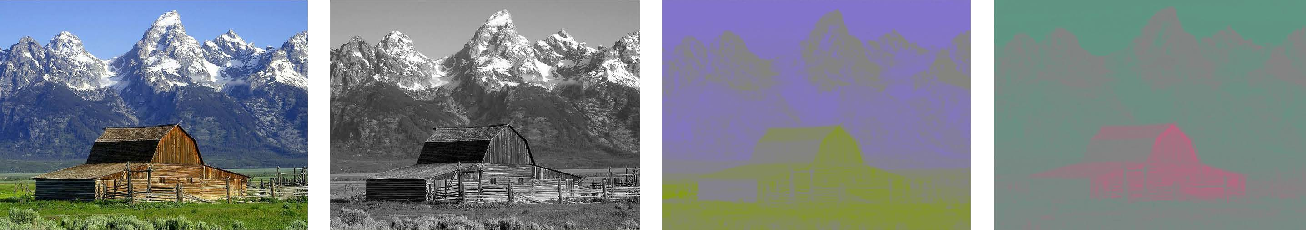
\includegraphics[width=\linewidth]{papers/jpeg/pictures/ycbcr.pdf}
    \caption{Von links Original, Luminanz, Chrominanz Blau/Gelb und Rot/Türkis
        \label{jpeg:fig:ycbcr}}
\end{figure}

Im Abschnitt \ref{jpeg:subsection:farbraumumrechnung} wurde beschrieben, dass die Farbauflösung der \(C_b\) und \(C_r\) für Menschen deutlich geringer ist wie in Abb. \ref{jpeg:fig:ycbcr} ersichtlich.
Dazu werden sie Tiefpass gefiltert, zudem üblicherweise vertikal und horizontal um den Faktor 2 unterabgetastet, was einer vierfachen Datenreduktion entspricht.
Die Farbunterabtastung bedeutet, dass jeder Pixel des Bild sein eigener Helligkeitswert behält, aber vier benachbarte Pixel sich die Farbinformationen teilen. 

\subsection{Tiling
\label{jpeg:subsection:tiling}}
Beim Tiling wird das Bild in jeweils \(8\times8\) Pixel grosse Blöcke unterteilt.
Da normalerweise die Seitenlängen eines Bildes sich nicht durch 8 teilen lässt, werden die Restlichen Zeilen bzw. Spalten jeweils aufgefüllt.
Wie das auffüllen geschieht ist im JPEG-Standard nicht festgelegt.
Eine gängige Methode ist das Wiederholen der letzte Pixel-Zeile oder -Spalte bis es aufgeht, wie in Abb. \ref{jpeg:fig:tiling} ersichtlich.
Auf diesen einzelnen Blöcken wird nun die DCT angewendet.

\begin{figure}
    \centering
    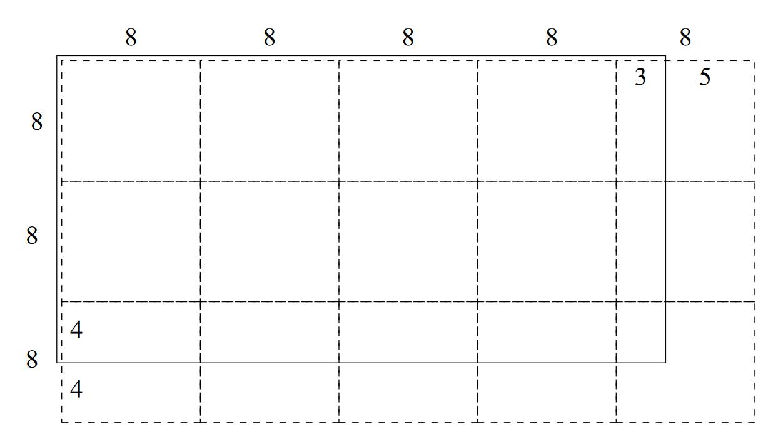
\includegraphics[width=90mm]{papers/jpeg/pictures/unterteilung.pdf}
    \caption{Bildeinteilung und Erweiterung
        \label{jpeg:fig:tiling}}
\end{figure}

\begin{table}[b]
    \centering
    \begin{tabular}{*{8}{r}}
        134.49 & 132.21 & 130.94 & 130.18 & 130.44 & 129.68 & 126.98 & 124.6\phantom{0}  \\
        137.73 & 137.73 & 138.85 & 139.71 & 138.73 & 134.44 & 127.84 & 122.32 \\
        148.5\phantom{0}  & 146.78 & 144.76 & 143.9\phantom{0}  & 142.36 & 137.31 & 131\phantom{.00}    & 126.14 \\
        155.37 & 150.22 & 143.14 & 138.57 & 136.55 & 135.79 & 133.58 & 132.72 \\
        153.04 & 148.47 & 141.88 & 138.08 & 135.54 & 134.78 & 132.79 & 131.07 \\
        146.95 & 145.43 & 144.16 & 142.64 & 140.86 & 136.3\phantom{0}  & 129.45 & 124.89 \\
        149.99 & 149.22 & 148.46 & 147.7\phantom{0}  & 144.74 & 138.07 & 129.47 & 123.85 \\
        160.7\phantom{0}  & 156.66 & 151.9\phantom{0}  & 147.7\phantom{0}  & 143.03 & 138.07 & 132.9\phantom{0}  & 128.61
    \end{tabular}
    \caption{Beispiel Originale Luminanzen eines 8x8 Pixelblocks
        \label{jpeg:tab:orgblock}}
\end{table}

\subsection{Quantisierung
\label{jpeg:subsection:quantisierung}}
Bei allen verlustbehafteten Komprimierungsverfahren entsteht die eigentliche Datenreduktion erst bei der Quantisierung.
Dazu werden die Koeffizienten aus der DCT Matrix \ref{jpeg:tab:dctblock} mit einer Quantisierungsmatrix elementweise dividiert und auf den nächsten ganzzahligen Wert gerundet.
Diese ist für die Qualität und der Menge der reduzierten Daten verantwortlich.
Die Quantisierung erfolgt mittels: 
\begin{equation}
    F^Q(x,y)
    =
    \operatorname{round} \left(
    \frac{F(x,y)}{Q(x,y)}
    \right)
\end{equation}
dabei ist \(F^Q\) die resultierende Matrix, \(F\) ist der transformierte Pixelblock und \(Q\) die Quantisierungsmatrix.
In \ref{jpeg:tab:quantblock} sind die Werte des Beispielblocks Quantisiert.
Bei diesem Schritt findet die Irrelevanzreduktion statt.
Irrelevanzreduktion meint die Daten zu entfernen die durch mathematische Modelle oder mittels empirische Werte als irrelevant gekennzeichnet sind.
Das ist z.B. wenn man ein Bild für Rot/Grün blinde Personen speichern möchte, wahlweise die Rot- oder Grün-Anteile speichert.
Da diese Personen sowieso nur einen Teil davon sehen können.

Das Auge ist empfindlicher auf hohe Farbunterschiede von benachbarten Pixel, das sind die tiefen Frequenzen in der DCT Matrix.
Daher werden diese weniger reduziert als die hohen, man sollte dafür eine optimale Tabelle verwenden.

Da der JPEG-Standard dies nicht vorgibt, muss die verwendete Tabelle im Header des Files mit abgelegt werden.
In Tabelle \ref{jpeg:tab:quant} ist eine gängige Quantiesierungstabelle für die Luminanz und eine für die Chrominanzen ersichtlich.

\begin{table}[t]
    \centering
    \begin{tabular}{*{8}{>{$}r<{$}}}
        1110.12 & 54.38  & -7.7\phantom{0}  & 9.19  & 0.3\phantom{0}   & 0.12  & 0.21  & -0.14 \\
        -27.43  & -15.67 & 0.12  & 0.19  & -0.19 & -0.02 & 0.09  & 0.18  \\
        -8.46   & -1.62  & -8.06 & -0.66 & -0.01 & 0.5\phantom{0}   & 0.08  & 0.43  \\
        -18.53  & -8.46  & -0.58 & -0.21 & -0.29 & -0.08 & 0.38  & 0\phantom{.00}    \\
        0.05    & 0.1\phantom{0}    & 15.43 & 0.02  & -0.13 & 0.31  & 0.07  & -0.35 \\
        -0.54   & -0.46  & 0.39  & 0.16  & 0.32  & -0.51 & 0.22  & 0.03  \\
        0.82    & 0.61   & 0.68  & 0.22  & 0.07  & -0.03 & 0.03  & 0.29  \\
        0.88    & 0.51   & -0.53 & 0.08  & 0.16  & 0.09  & -0.37 & -0.1\phantom{0} 
    \end{tabular}
    \caption{Beispiel 8x8 Pixelblock der Originalwerte nach der DCT
        \label{jpeg:tab:dctblock}}
\end{table}

\begin{table}[]
    \centering
    \begin{tabular}{*{8}{>{$}r<{$}}}
        69 & 5  & -1 & 1  & 0  & 0  & 0  & 0 \\
        -2 & -1 & 0  & 0  & 0 & 0 & 0  & 0  \\
        -1 & 0 & -1 & 0 & 0 & 0  & 0  & 0  \\
        -1 & 0 & 0 & 0 & 0 & 0 & 0  & 0 \\
        0  & 0  & 0  & 0  & 0 & 0  & 0  & 0 \\
        0 & 0 & 0  & 0  & 0  & 0 & 0  & 0  \\
        0  & 0  & 0  & 0  & 0  & 0 & 0  & 0  \\
        0  & 0  & 0 & 0  & 0  & 0  & 0 & 0
    \end{tabular}
     \caption{Beispiel 8x8 Pixelblock der quantisierten DCT Werte
        \label{jpeg:tab:quantblock}}
\end{table}

\begin{table}[b]
    \centering
    \begin{tabularx}{0.47\linewidth}{|X|X|X|X|X|X|X|X|}
        \hline
        16 & 11 & 10 & 16 & 24  & 40 & 51 & 61    \\ \hline
        12 & 12 & 14 & 19 & 26  & 58 & 60 & 55    \\ \hline
        14 & 13 & 16 & 24 & 40  & 57 & 69 & 56    \\ \hline
        14 & 17 & 22 & 29 & 51  & 87 & 80 & 62    \\ \hline
        18 & 22 & 37 & 56 & 68  & 109 & 103 & 77  \\ \hline
        24 & 35 & 55 & 64 & 81  & 104 & 113 & 92  \\ \hline
        49 & 64 & 78 & 87 & 103 & 121 & 120 & 101 \\ \hline
        72 & 72 & 95 & 98 & 112 & 100 & 103 & 99  \\ \hline        
    \end{tabularx}
    \qquad
    \begin{tabularx}{0.47\linewidth}{|X|X|X|X|X|X|X|X|}
        \hline
        17 & 18 & 24 & 47 & 99 & 99 & 99 & 99  \\ \hline
        18 & 21 & 26 & 66 & 99 & 99 & 99 & 99  \\ \hline
        24 & 26 & 56 & 99 & 99 & 99 & 99 & 99  \\ \hline
        47 & 66 & 99 & 99 & 99 & 99 & 99 & 99  \\ \hline
        99 & 99 & 99 & 99 & 99 & 99 & 99 & 99  \\ \hline
        99 & 99 & 99 & 99 & 99 & 99 & 99 & 99  \\ \hline
        99 & 99 & 99 & 99 & 99 & 99 & 99 & 99  \\ \hline
        99 & 99 & 99 & 99 & 99 & 99 & 99 & 99  \\ \hline  	  
    \end{tabularx}
    \caption{Beispiel Quantisierungstabelle für Luminanz (links) und Chominanzen
        \label{jpeg:tab:quant}}
\end{table}



\subsection{Umsortierung und Differenzkodierung
\label{jpeg:subsection:umsortierung}}
Die 64 Koeffizienten des Pixelblocks werden nach der Quantisierung im Zig-Zag Muster abgetastet wie in Abb. \ref{jpeg:fig:zigzag} zeigt.
Die linke obere Ecke ist der Gleichanteil (DC-Wert), das ist die mittlere Helligkeit des Blocks.
Der Rest ist der Wechselanteil (AC-Wert), wenn man dem Zig-Zag folgt erreicht man den mit der höchsten Frequenz zuletzt.

Die Koeffizienten mit hohem Wert (die niedrigen Frequenzen) stehen nun am Anfang und die kleine Koeffizienten weiter hinten.
Je stärker quantisiert wurde, desto mehr Nullen sind am Ende, was für eine Lauflängenkodierung optimal ist.

\begin{figure}
    \centering
    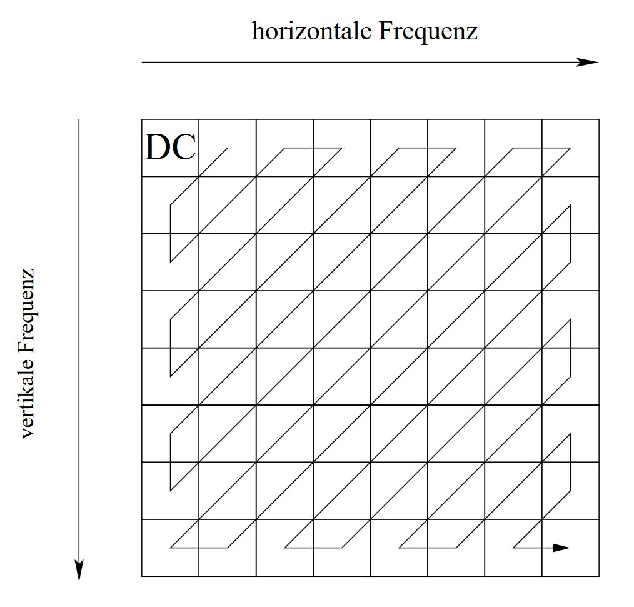
\includegraphics[width=62mm]{papers/jpeg/pictures/zigzag.pdf}
    \caption{Zig-Zag Abtastung der Koeffizienten
        \label{jpeg:fig:zigzag}}
\end{figure}

Der DC-Wert und die AC-Werte werden getrennt behandelt.
Der Grund dafür liegt darin, dass Bilder oft grössere, fast gleichfarbige Flächen besitzen.
Dadurch haben benachbarte Blöcke ähnliche Gleichanteile (der Mittelwert eines Blocks), die differenziell kodiert werden.

Das bedeutet, man betrachtet nicht jeden DC-Wert einzeln, sondern die Differenzen zwischen den Blöcken.
Die Differenzkodierung beginnt mit dem zweiten Block des Bildes.
Durch die Differenzbildung wird der kodierte Wert kleiner, damit benötigt man weniger Bits.

Wenn an dem Beispiel in Tabelle \ref{jpeg:tab:quantblock} die differenzielle Kodierung angewendet wird, wird vom DC-Wert 69 der Wert des vorherigen Blocks (76) abgezogen \(69-76 = -7\).

\subsection{Entropiekodierung
\label{jpeg:subsection:entropiekodierung}}
Der differenzkodierte Gleichanteil wird direkt mit einem Huffmantree kodiert.
Um Speicherplatz zu reduzieren, werden die AC-Werte zuerst einer run length coding (RLC) unterzogen.
Diese verschlüsselt ein Huffmantree anschliessend.
In Abb. \ref{jpeg:fig:huffman} sind die Bäume dargestellt.
Der Huffmantree ist im JPEG-Standard nich vorgegeben und muss deshalb im File header hinterlegt werden.

Die RLC der Wechselanteile erfolgt in einer Klammer-Sortierung.
Der erste Wert gibt an, wie viele AC-Werte Null sind vor dem, der kodiert werden soll und der zweite Wert in der Klammer die Anzahl der Bits für die Kodierung.
Darauf folgt der eigentliche AC-Wert selbst also 
\begin{equation}
    [(0,3)5],[(0,2)-2], \dots, [(2,1)-1], EOB.
    \label{jpeg:equation:kette}
\end{equation}
Nach dem letzten Wert \(\neq 0\) wird als Abschluss der End-of-Block (EOB) hinzugefügt der als (0,0) definiert ist.

\begin{figure}[t]
    \centering
    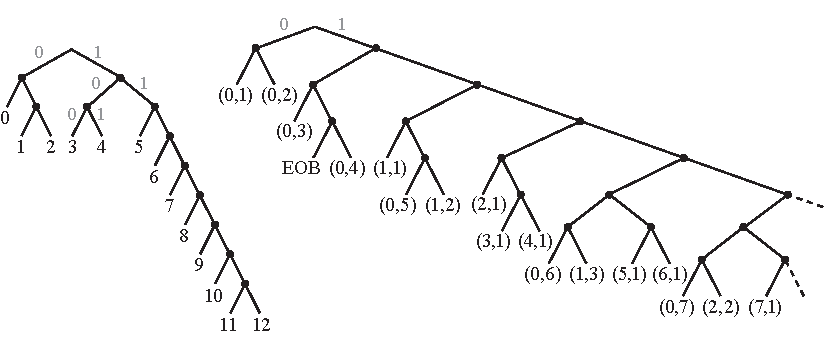
\includegraphics[width=\textwidth]{papers/jpeg/pictures/huffman.pdf}
    \caption{Huffman-Baum für DC-Wert(links) und AC-Wert als Dupel 
        \label{jpeg:fig:huffman}}
\end{figure}

Die Huffman Kodierung zweigt von jedem Knoten nach links 0 und nach rechts 1.
Um z.B. den Wert 4 zu erhalten, braucht man die Bitfolge 101.
Um mittels der Kodierung den verschlüsselten Wert zu erhalten, muss man bei jedem Knoten weiter gehen, bis man im Huffmantree ein Ende erreicht (z.B. 1110 entspricht 6).

Nun kann man mit Hilfe der Tabelle \ref{jpeg:tab:huffman} und den Bäumen den Bitstream für diesen Pixelblock erstellen.
Der DC-Wert \(-7\) hat laut Tabelle \ref{jpeg:tab:huffman} die binäre Länge 3.
Aus dem Baum gemäss Abb. \ref{jpeg:fig:huffman} ergibt sich dafür 100.
Aus der Tabelle \ref{jpeg:tab:huffman} liest man für den Wert \(-7\) den binären Wert 000.
Die binäre Länge 100 und der binäre Wert von \(-7\) mit 000 wird zusammen als 100000 geschrieben.

Für die AC-Werte werden nun die Kette \eqref{jpeg:equation:kette} aus der RLC mit dem Baum gemäss Abb. \ref{jpeg:fig:huffman} in Bits umgewandelt.
Beispiel: Der Klammerausdurck \([(0,3)5]\) am Anfang der Kette in \eqref{jpeg:equation:kette} hat aus dem Baum den Wert 100 und die 5 gemäss Tabelle \ref{jpeg:tab:huffman} als binären Wert 101, was 100101 ergibt.
Werden alle Werte der Kette \eqref{jpeg:equation:kette} so verarbeitet, erhält man
\begin{equation}
    100000'100101'01'01'000'000'000'001'111000'111000'1010    
\end{equation}
als Bitstream.
Die ersten 6 Bits sind aus dem DC-Wert der Rest aus dem AC teil.

Der Bitstream besteht aus 44 Bits.
Hätte man die Werte aus Tabelle \ref{jpeg:tab:quantblock} genommen bräuchte, man \(8\times8\times8=512\) Bits, aus 8x8 Einträgen mit jeweils 8 Bit Länge, was dem 11-fachen entspricht.

\begin{table}[t]
    \centering
    \begin{tabular}{l>{$}c<{$}l}
        Länge & \textrm{Eintrag}                     & Binär\\
        0     & 0                           		 & \(-\) \\
        1     & -1,1                         	 	 & 0,1 \\
        2     & -3,-2,2,3                   		 & 00,01,10,11 \\
        3     & -7,-6,-5,-4,4,5,6,7         		 & 000,001,010,011,100,101,110,11 \\
        4     & -15,-14,\dots,-8,8,\dots,15          & 0000,0001,\dots,0111,1000,\dots,1111 \\
        5     & \dots                                & \dots \\
        6     & \dots                                & \dots                           
    \end{tabular}
    \caption{Beispiel für eine Huffman-Code-Tabelle
        \label{jpeg:tab:huffman}}
\end{table}

\subsection{Probleme JPEG
\label{jpeg:subsection:probleme}}
Wenn man ein Bild zu stark komprimiert, treten Artefakte auf.
Artefakte zeigen sich bei Bildern als kleine Klötzchen wie in Abb. \ref{jpeg:fig:blockart} erkennbar.
Die Ursache dafür ist das zu starke Quantisieren der 8x8 Pixelblöcke nach der DCT.
Dadurch gehen zu viele Daten verloren und der gesamte Block besitzt dieselbe Farbe.

Für die Text- und Fingerprint-Kompression eignet sich der JPEG-Standard nicht.
Texte und Fingerprints haben Typischerweise harte Pixelübergänge.
Für die eindeutige Erkennung eines Fingerprints darf seine Struktur nicht verändert werden.

Die Abb. \ref{jpeg:fig:textart} zeigt, was mit komprimiertem Text passiert.
Bei Abb. \ref{jpeg:fig:fingerprint} ist die linke Hälfte unkomprimiert und die rechte im JPEG-Format komprimiert .



\begin{figure}[h]
    \centering
    \subfigure[Textartefakt\label{jpeg:fig:textart}]{
        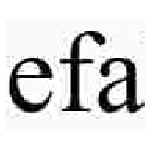
\includegraphics[width=0.34\textwidth]{papers/jpeg/pictures/artifakte.pdf}}
    \hfill
    \subfigure[Fingerprint\label{jpeg:fig:fingerprint}]{
        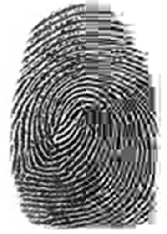
\includegraphics[width=0.28\textwidth]{papers/jpeg/pictures/fingerprint.pdf}}
    \hfill
    \subfigure[Blockartefakte\label{jpeg:fig:blockart}]{
        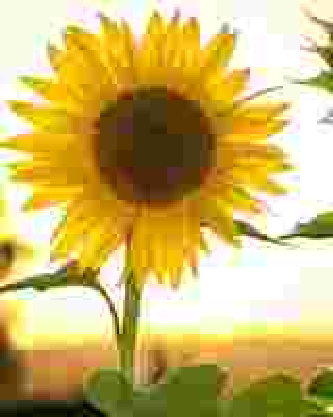
\includegraphics[width=0.32\textwidth]{papers/jpeg/pictures/sonnenblume.pdf}}
    \caption{Verschiedene Artefakte von JPEG 
    \label{jpeg:fig:bspproblem}}
\end{figure}
